\section{Evaluering}
\subsection{Test af Korrekthed}
Vi har som i \des løbende skrevet test før vi implementerede hver ny funktion i \code{RTP}-versionen.  Tabellen herunder viser testresultaterne for de test der er lavet specifikt for \code{RTP}-versionen.
\begin{longtable}{lr}
   	\toprule
    \mc{Test} & \mc{Resultat} \\
    \midrule
    \endfirsthead 
    \toprule
    \mc{Test} & \mc{Resultat} \\
    \midrule
    \endhead % slut efterfølgende headere
    \bottomrule
    \multicolumn{2}{r}{\textit{fortsættes}}
    \endfoot % slut footer
    \bottomrule
    \endlastfoot % slut sidste footer
test\_Alternation  & ok\\
test\_AlternationChoiseReader  & ok \\
test\_AlternationChoiseWriter  & ok \\
test\_AlternationExecuteReadDeadline  & ok\\
test\_AlternationExecuteSkipDeadline  & ok\\
test\_AlternationExecuteTimeoutDeadline  & ok \\
test\_AlternationExecuteWriteDeadline  & ok \\
test\_Alternationchoise1Deadline  & ok \\
test\_Alternationchoise2Deadline  & ok \\
test\_ChoisemultipleReader  & ok \\
test\_ChoisemultipleReader2  & ok \\
test\_ChoisemultipleWriter  & ok\\
test\_PoisonAndDeadline1  & ok\\
test\_PoisonAndDeadline2  & ok\\
test\_Reader\_Inheritance  & ok\\
test\_RetireAndDeadline  & ok\\
test\_Writer\_Inheritance  & ok\\
test\_channelpriority\_from\_low\_deadline  & ok\\
test\_channelpriority\_from\_low\_deadline2  & ok\\
test\_channelpriority\_from\_no\_deadline  & ok\\
test\_channelpriority\_from\_no\_deadline2  & ok\\
test\_readDeadline  &ok\\
test\_writeDeadline  & ok\\
test\_xreset\_inheritance  & ok\\
test\_xreset\_inheritance\_from\_two\_step  & FAIL\\
\end{longtable}


 Alle test med en undtagelse fungerer korrekt. Testen der fejler hedder test"_xreset"_inheritance"_from"_two"_step, og viser en situation hvor den samme proces får løftets sin prioritet to gange i træk, først med en høj prioritet, og efterfølgende med en mellemprioritet. Efterfølgende skal processen sænke sin prioritet, først til  mellemprioriteten og tilslut til sin originale prioritet. Her viser det sig vi har lavet en fejl i implementeringen, således at prioriteten ikke bliver nedsat til mellemprioriteten. \CRef{fig:priority-inheritance} viser prioriteten mens processen bliver op og nedprioriteret. Tiden har ikke tilladt os at løse problemet, men  kan løses ved at kræve at, når en proces opprioriteres gemmes hvilken proces der står bag, så når en proces ønsker at fjerne sin opprioritering fra andre processer er det kun sin egen  prioritet den fjerner.  
 
  
\begin{figure}
 \begin{center}
  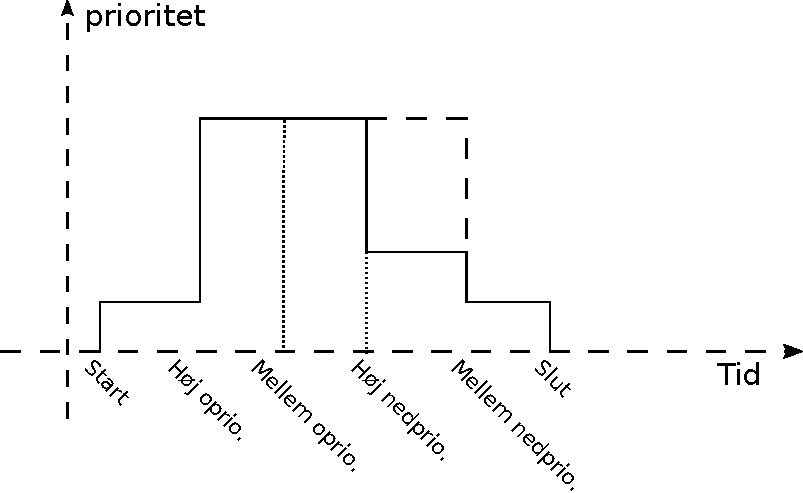
\includegraphics[scale=1]{images/priority-inheritance}
	\caption{Figuren viser hhv. forventet og faktisk prioritetsarvning. Der hvor den faktiske og forventede opførsel adskiller sig er forventet den fuldt optrukne streg, mens den stiplede streg er den faktiske opførsel.}
	\label{fig:priority-inheritance}
\end{center}
\end{figure}
  

\subsection{Slagterieksempel}

Ved at basere koden på \pycsp kan netværket nemt udvides hvis de fysiske rammer for slagteriet ændre sig. Viser det sig f.eks at kameraet holder den samlede produktivitet af netværket tilbage kan, slagteriet tilføjet endnu et kamera, og nemt udvide procesnetværket med endnu en kameraproces, som kan arbejde samtidigt med det første kamera. 


Selvom \pycsp kan udnytte et vilkårligt antal processorer i en computer, så længe der er flere processer end processorer, vil man se ændring i ydelsen hvis man variere  antallet af processer. Med \code{RTP}-versionen kan man nemt ændrer på antallet af konvertering- og analyse-processer for at fintune applikationen og  udnytte den underliggende platform. \code{RTP}-versionen sikrer i modsætning til \code{greenlets}-versionen at netværket hele tiden har fokus på først at videresende grisene nærmest robotten. \CRef{fig:pig-network3} viser hvordan netværket kan se ud med flere konverterings og analyse processer. 

\begin{figure}
 \begin{center}
  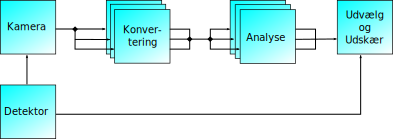
\includegraphics[scale=1]{images/pig-network3}
	\caption{Procesnetværk med flere konverteringsprocesser, og analyseprocesser}
	\label{fig:pig-network3}
\end{center}
\end{figure}

Ved implementering af slagterieksemplet i \code{RTP}-versionen, slipper de enkelte processer for at holde styr på tiden, og foretage sammenligningen om den enkelte gris deadline er overskredet. Når de modtager en gris sætter de deres egen deadline til grisens via funktionen \code{Set\_deadline}.  Hver proces skal til gengæld kunne håndtere at modtage en \code{DeadlineException}, som de i dette tilfælde blot kan håndteres ved at smide den nuværende gris væk, da den ikke længere er relevant, og  gå i gang med modtage en ny gris.

I \code{greenlets}-versionen kom vi ind på at processerne frivilligt skal afgive kontrollen, før robotten kan foretage udskæringen, men at der ikke findes en metode til midlertidigt at afgive kontrollen. Med \code{RTP}-versionen og funktionen \code{Release} har alle processer mulighed for med jævne mellemrum at afgive kontrollen så robotten rettidigt kan foretage selve udskæringen. Hermed skal vi ikke introducere en delt datastruktur, med de problemer den introducere og som vi snakkede om i afsnittet Barrierer på side \pageref{sec:barrierer}.
  
Ved at basere RTP på  på \code{greenlets}-versionen, kan kun en proces  kan være aktiv på samme tid. Dermed kan vi kun udnytte en processor, som  passer dårligt sammen med denne applikation, hvor man vil forvente at det endelige program vil skulle køre på en supercomputer, med mange processorer for at kunne processere grisene inden de skal udskæres.  Den eneste metode der findes til samtidig behandling af flere processer i  de versioner, der baserer sig på \code{greenlets}-versionen, er at anvende en \code{IO}-dekorering. Denne dekorering placerer en funktion i en separat tråd, så flere funktioner kan køre samtidigt. Man skal her dog være opmærksom på at GIL'en stadig forhindre paralleludførsel. Eventuel parallel udførsel vil derfor kræve at koden i IO dekoreringen, kalder eksterne moduler som diskuteret i \cref{chap:csp}. Et propblem ved at køre flere funktioner samtidigt er det operativsystemets \sched, der står for planlægningen og udførslen af funktionerne, uden at kende noget til vores interne planlægning. En brug af \code{IO}-dekorering og eksterne moduler til at sikre samtidighed skal derfor bruges med varsomhed og kun efter en analyse af den enkelte applikation, da samtidige processer på den samme processor vil kæmpe mod hinanden om processorresurser.


 
